\subsection{Upstream training with random labels}\label{sec:randlabel}
\textbf{Q1 (open question [\citenum{randlabel}]).} {When trained with random labels upstream followed by true labels downstream, the test performance of a DNN with ReLUs degrades, Why?}

\textbf{Setup to answer Q1.} We hypothesise that the answer to the above question lies in the gates. To test our hypothesis, we train in two phases (i) Phase I: upstream training with label noise levels $\gamma=0, 25\%, 50\%, 75\%$ and (ii) Phase II: downstream training with true labels. For $\gamma=0$ there is no Phase II because Phase I is already with true labels. We then measure the information stored in the gates at the end of each of the two phases. To this end, we consider the DGN setup in \Cref{fig:dgn-prior-new} (left), and train the feature network (which is a DNN with ReLUs) with $\hat{y}_{\text{f}}$ as output node. In Phase I, we train the feature network for different values of label noise $\gamma=0, 25\%, 50\%, 75\%$, which gives us models $M1(\gamma)$ (see \Cref{fig:rand-label-setup}). To measure the information in the gates learnt at the end of Phase I, we keep these gates fixed and train the value network with true labels -- this gives us models $M2(\gamma)$ (see \Cref{fig:rand-label-setup}). In Phase II, we start with models $M1(\gamma)$ (i.e., obtained at end of Phase I), and perform downstream training with true labels to obtain models $M4(\gamma)$.  To measure the information in the gates learnt at the end of Phase II, we keep these gates fixed and train the value network with true labels -- this gives us models $M5(\gamma)$ (see \Cref{fig:rand-label-setup}).

\begin{figure}[t]
\centering
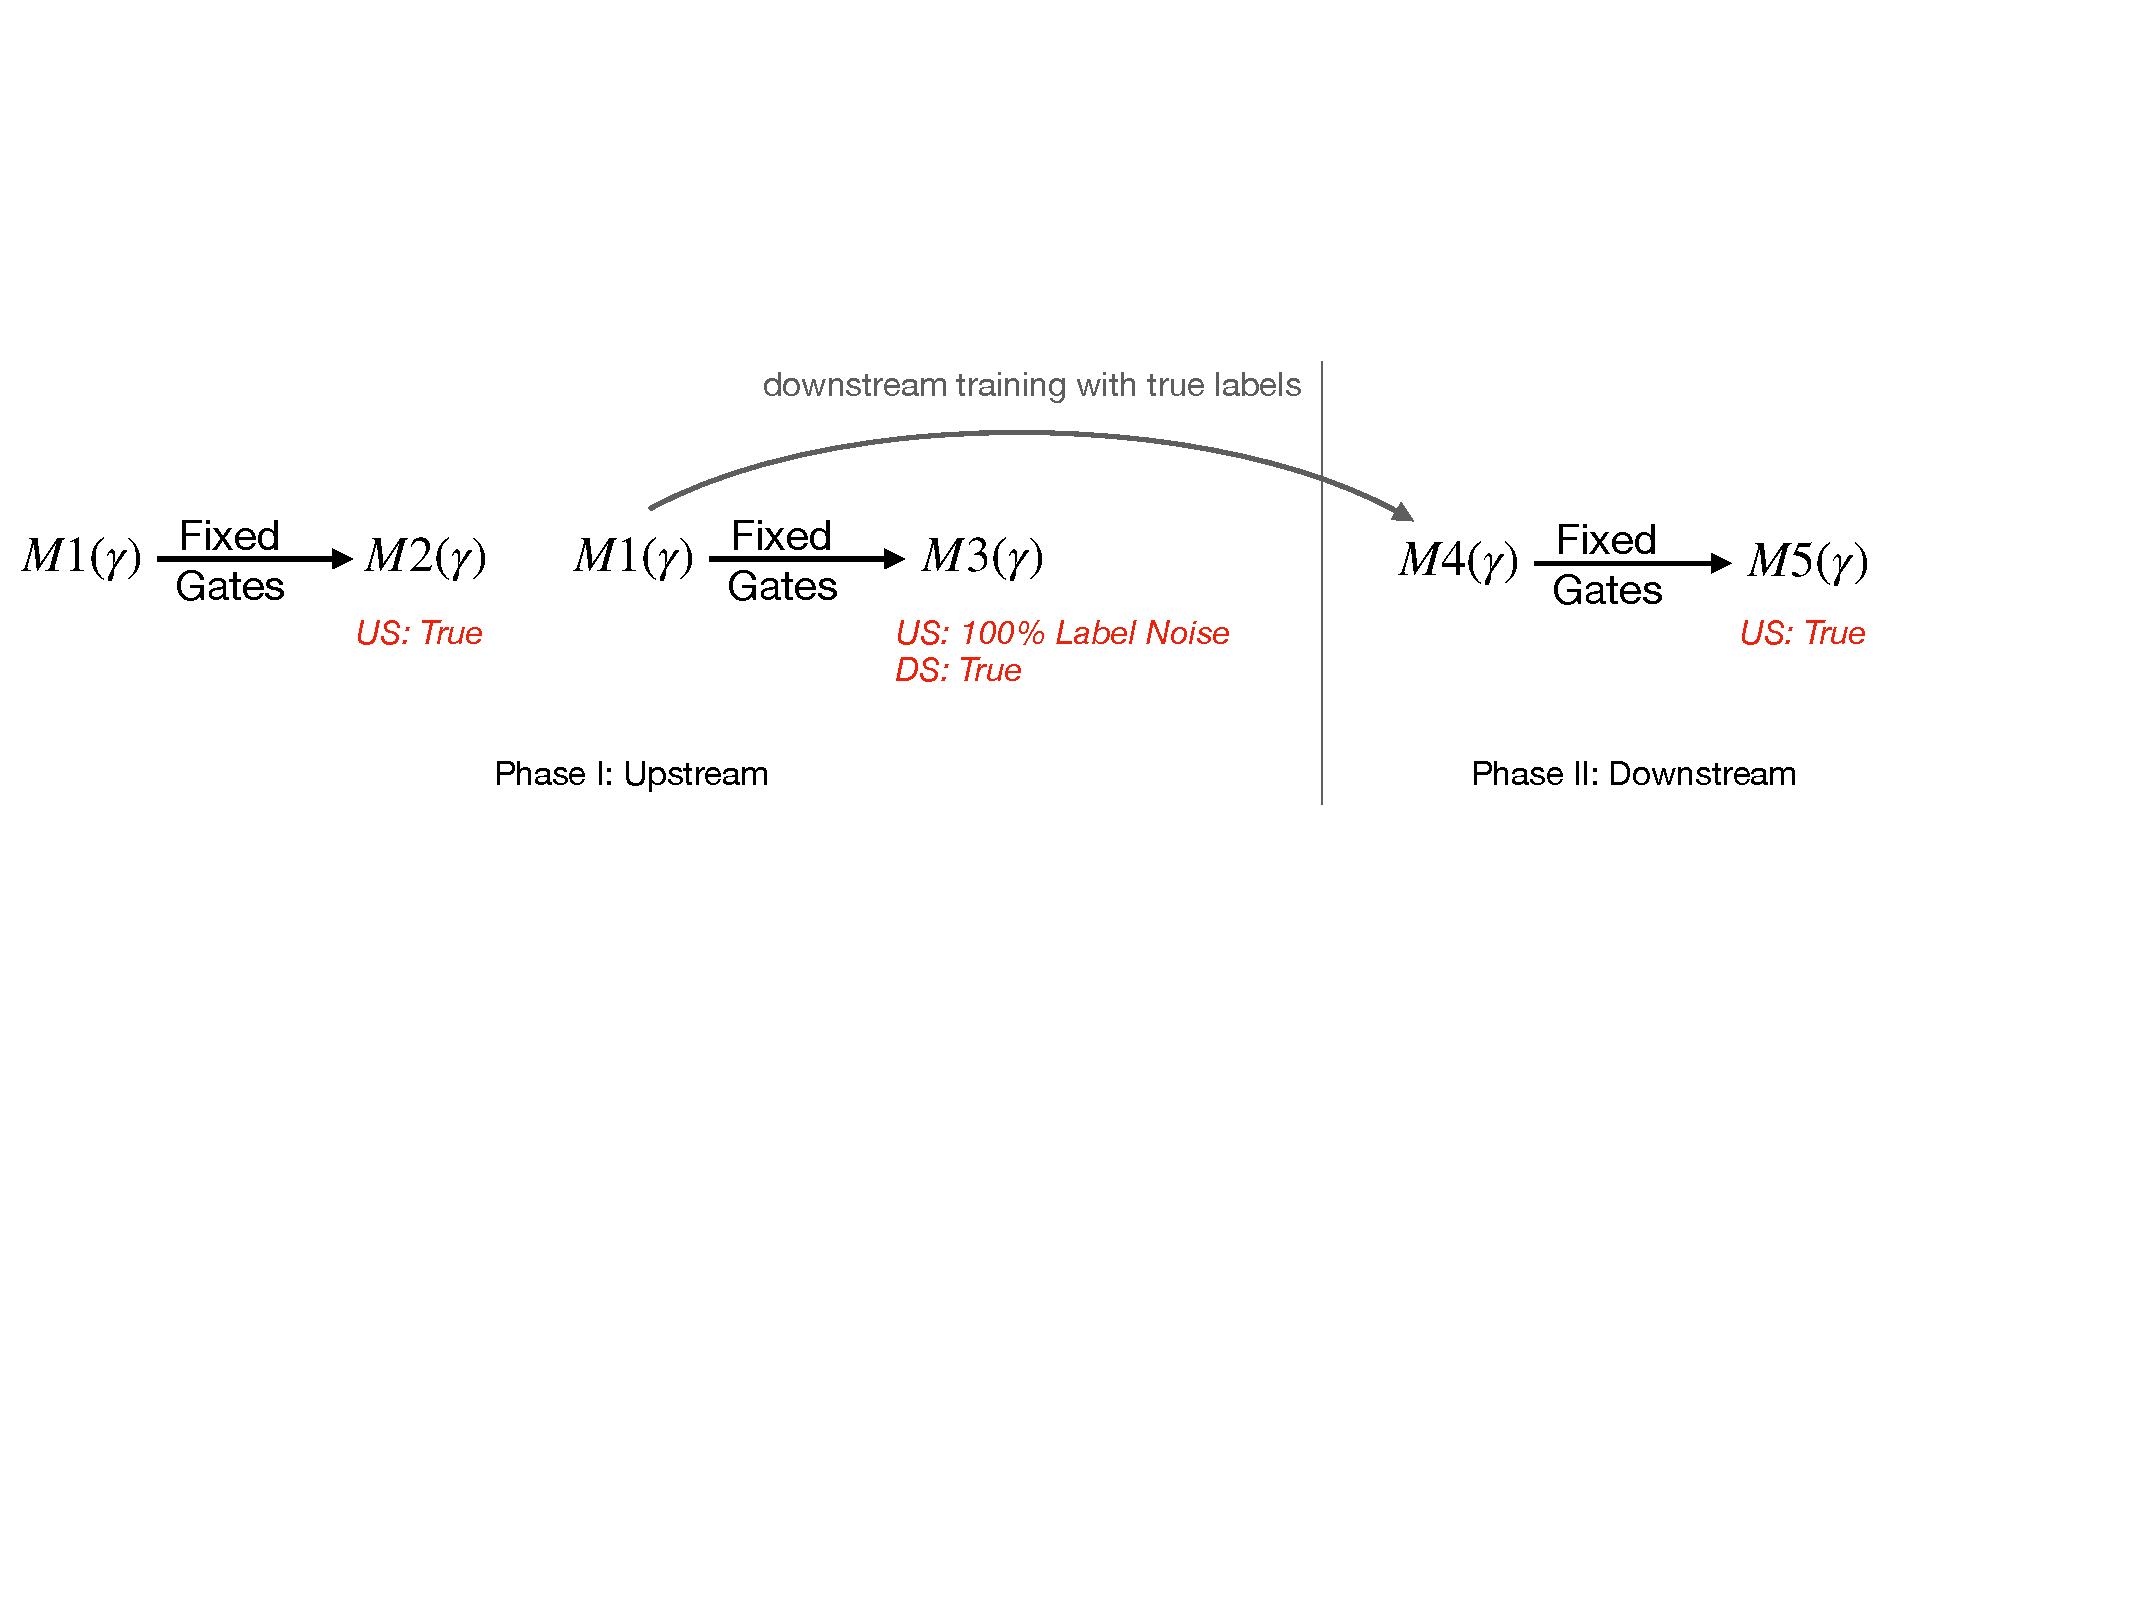
\includegraphics[scale=0.25]{figs/rand-label-big.pdf}
\caption{\small Shows various models trained in Experiment 2. Here, US and DS stand for upstream and down stream respectively. True for training with true labels. Here models $M1$ and $M4$ are feature networks (DNNs with ReLUs), and $M2, M3$ and $M5$ are value networks which use the fixed gates from the feature networks. Models are parameterised by $(\gamma)$ which is the label noise level.}
\label{fig:rand-label-setup}
\end{figure}


\textbf{Q2 (new question).} {When trained with random labels upstream followed by true labels downstream, \emph{if the gates are fixed throughout and only the weights are trained}, does the test performance degrade?}

\textbf{Setup to answer Q2.} Here, we pick up the models trained at the end of Phase I, use them as feature networks and fix the gates. We then train the value network, first upstream with with $100\%$ random labels, and then downstream with $100\%$ true labels--this gives us models $M3(\gamma)$.

The results of the experiments with random labels shown in \Cref{tb:rand-label} (plots are in the Appendix).

\textbf{Answer to Q2.} \emph{When the gates are fixed test performance is robust to upstream training with random labels.} In  \Cref{tb:rand-label}, look at the performance of $M3(\gamma=0)$ and compare it with performance of  $M4(\gamma), \gamma=25,50,75$. When the gates are fixed, i.e., in $M3(0)$ (note: this is a value network), the upstream training with even $100\%$ label noise does not hurt the test performance so much ($81.2-79.3 <2\%$) in comparison to the cases when the gates are allowed to change, i.e., $M4(\gamma)$ (note: these are feature networks), the test performance degrades (from $81.2$) to $76.9$ ( $ 4.3\%$ for $\gamma=25$), $73.6$ ( $7.6\%$ for $\gamma=50$) and  $68.1$ ($13.1\%$ for $\gamma=75$) for even less than $100\%$ label noise.
%\begin{comment}
\begin{table}[b]
\centering
\resizebox{0.9\columnwidth}{!}{
\begin{tabularx}{\columnwidth}{c *{6}{Y}}
\toprule
 & \multicolumn{4}{c}{Phase I: Upstream}  
 & \multicolumn{2}{c}{Phase II: Downstream}\\
\cmidrule(lr){2-5} \cmidrule(l){6-7}
&  \multicolumn{2}{c}{ReLU}  &\multicolumn{2}{c}{Fixed Gates} & ReLU & {Fixed Gates}\\
\cmidrule(lr){2-3} \cmidrule(lr){4-5}\cmidrule(lr){6-7}
$\gamma$& Best & End & True& US\&DS & True & True\\\hline\arrayrulecolor{white}\midrule
0 &{\bf{81.2}}{\tiny $\pm$ 0.3} & 80.0{\tiny $\pm$ 0.4} &{\bf{80.3}}{\tiny $\pm$ 0.2} & {\bf{79.3}}{\tiny $\pm$ 0.4} &-&- \\\hline\hline
{25}&76.1{\tiny $\pm$ 0.6} & 63.1{\tiny $\pm$ 0.7}& 74.7{\tiny $\pm$ 0.5}& 72.3{\tiny $\pm$ 0.2}&76.9{\tiny $\pm$ 0.1}&76.9{\tiny $\pm$ 0.4}\\\hline\hline
{50}&70.9{\tiny $\pm$ 0.8} & 41.5{\tiny $\pm$ 1.1}& 69.9{\tiny $\pm$ 0.3} & 66.8{\tiny $\pm$ 0.1}&73.4{\tiny $\pm$ 0.3}&73.6{\tiny $\pm$ 0.4}\\\hline\hline
{75}&56.9{\tiny $\pm$ 0.4} & 23.4{\tiny $\pm$ 0.4}& 63.9{\tiny $\pm$ 0.4} &60.0{\tiny $\pm$ 0.3}&68.1{\tiny $\pm$ 0.4}&67.7{\tiny $\pm$ 0.6}\\\hline
\arrayrulecolor{black}\bottomrule
Models & \multicolumn{2}{c}{M1($\gamma$)} & M2($\gamma$) & M3($\gamma$)& M4($\gamma$) & M5($\gamma$)\\\bottomrule
\end{tabularx}
}
\caption{\small Shows the $\%$ test accuracy (on test data with true labels) of the models in Experiment 2 on CIFAR-10. The numbers are averaged over $3$ runs (best accuracy is taken in each run except for column `End'). For column `End', in each run the average test accuracy over the last $10$ epochs are considered. Optimiser: Adam(3e-4).}
\label{tb:rand-label}
\end{table}
%\end{comment}
\begin{comment}
\begin{table}[t]
\begin{tabularx}{\columnwidth}{c *{6}{Y}}
\toprule
 & \multicolumn{2}{c}{Phase I} &  \multicolumn{2}{c}{Phase I End} &{Phase II}&  \multicolumn{1}{c}{Phase II End}\\
\cmidrule(lr){2-3} \cmidrule(lr){4-5} \cmidrule(l){6-6}\cmidrule(l){7-7}
&  \multicolumn{2}{c}{ReLU}  &\multicolumn{2}{c}{Fixed Gates} & ReLU &  \multicolumn{1}{c}{Fixed Gates }\\
\cmidrule(lr){2-3} \cmidrule(lr){4-5} \cmidrule(l){6-6}\cmidrule(l){7-7}
$\gamma$& Best & End & True& US/DS & True & True\\\hline\arrayrulecolor{white}\midrule
0 &{\bf{81.2}}{\tiny $\pm$ 0.3} & 80.0{\tiny $\pm$ 0.4} &{\bf{80.3}}{\tiny $\pm$ 0.2} & {\bf{79.3}}{\tiny $\pm$ 0.4} &-&- \\\hline\hline
{25}&76.1{\tiny $\pm$ 0.6} & 63.1{\tiny $\pm$ 0.7}& 74.7{\tiny $\pm$ 0.5}& 72.3{\tiny $\pm$ 0.2}&76.9{\tiny $\pm$ 0.1}&76.9{\tiny $\pm$ 0.4}\\\hline\hline
{50}&70.9{\tiny $\pm$ 0.8} & 41.5{\tiny $\pm$ 1.1}& 69.9{\tiny $\pm$ 0.3} & 66.8{\tiny $\pm$ 0.1}&73.4{\tiny $\pm$ 0.3}&73.6{\tiny $\pm$ 0.4}\\\hline\hline
{75}&56.9{\tiny $\pm$ 0.4} & 23.4{\tiny $\pm$ 0.4}& 63.9{\tiny $\pm$ 0.4} &60.0{\tiny $\pm$ 0.3}&68.1{\tiny $\pm$ 0.4}&67.7{\tiny $\pm$ 0.6}\\\hline
\arrayrulecolor{black}\bottomrule
Models & \multicolumn{2}{c}{$M1(\gamma)$} & $M2(\gamma)$ & $M3(\gamma)$& $M4(\gamma)$ & $M5(\gamma)$\\\bottomrule
\end{tabularx}
\caption{\small Shows the $\%$ test accuracy (on test data with true labels) of the various models in Experiment 2 on CIFAR-10. The numbers are averaged over $3$ runs (best accuracy is taken in each run except for column `End'). For column `End', in each run the average test accuracy over the last $10$ epochs are considered. Optimiser: Adam(3e-4). The plots are in the Appendix.}
\label{tb:rand-label}
\end{table}
\end{comment}

\textbf{Answer to Q1.} \emph{The test performance degrades because the gates get degraded.} This follows from the fact that the performance of the DNN with ReLUs after training with true labels in Phase II, i.e., $M4$ and that of the value network with the fixed gates at end of Phase II, i.e., $M5$ are approximately equal (within $0.5\%$). In short, $M5$ gates come from $M4$.

\textbf{Gates are fairly robust to random labels.} Note that while training with random labels upstream, the test performance initially improves, reaches a peak and then degrades (see columns `Best' and `End' in \Cref{tb:rand-label}). The performance of the DNN with ReLUs at the end of `Phase I' is shown in the column `End' of \Cref{tb:rand-label}. However, the performance of the fixed gates at the end of `Phase I' shown in fourth column of \Cref{tb:rand-label} i.e., $M2(\gamma)$, is much better and is more closer to the performance of the downstream models $M4(\gamma)$. This means, during upstream training with random labels, the performance degradation post the `Best' value mostly affects only the weights and not the gates.

\begin{comment}
\begin{figure}[h]
\begin{minipage}{0.99\columnwidth}
\resizebox{\columnwidth}{!}{
\begin{tabular}{ccc}
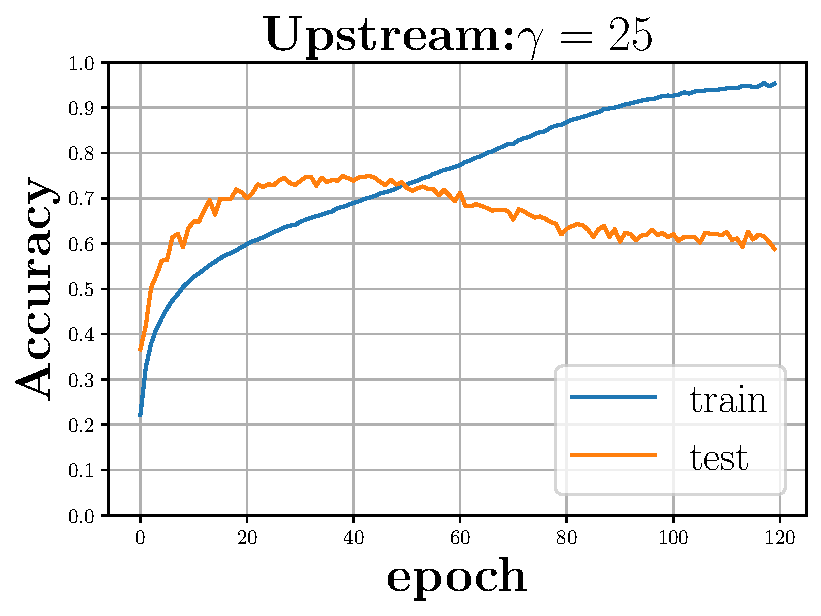
\includegraphics[scale=0.125]{figs/relu_25.pdf}&
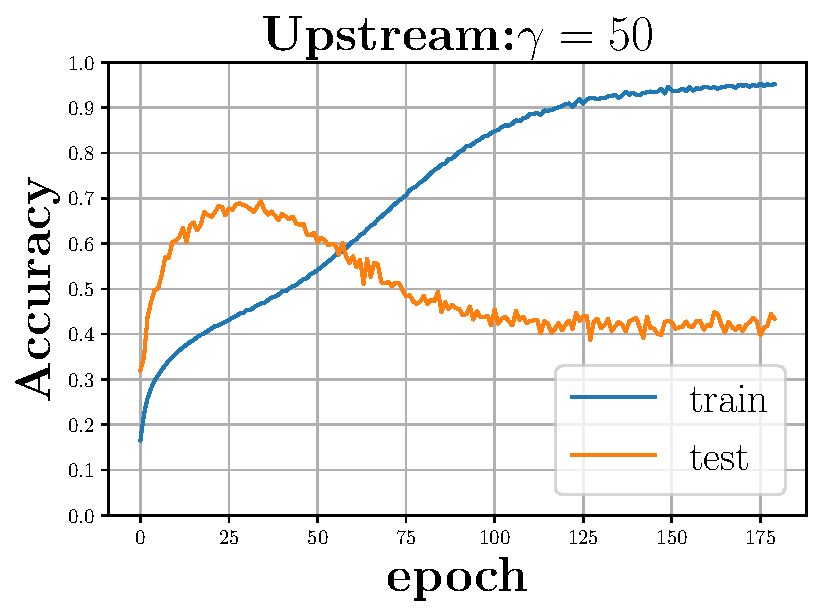
\includegraphics[scale=0.125]{figs/relu_50.pdf}&
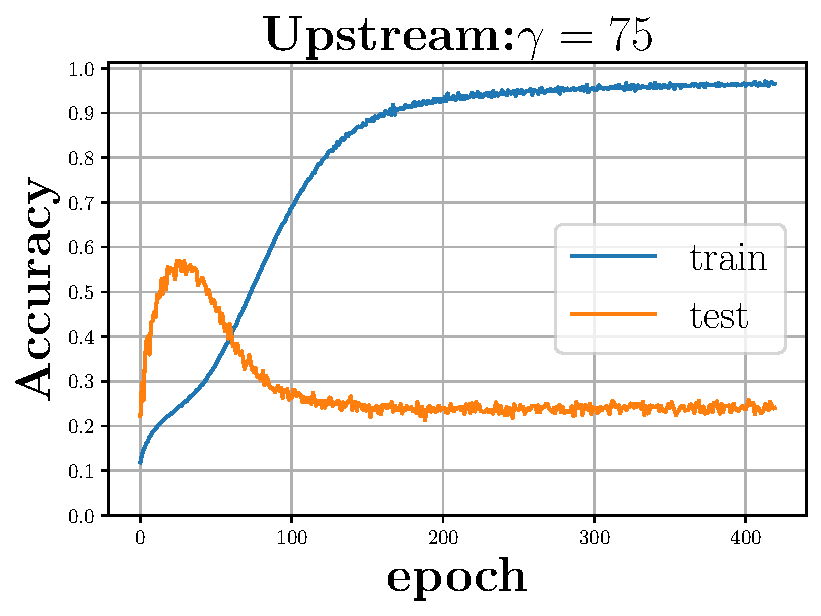
\includegraphics[scale=0.125]{figs/relu_75.pdf}
\\
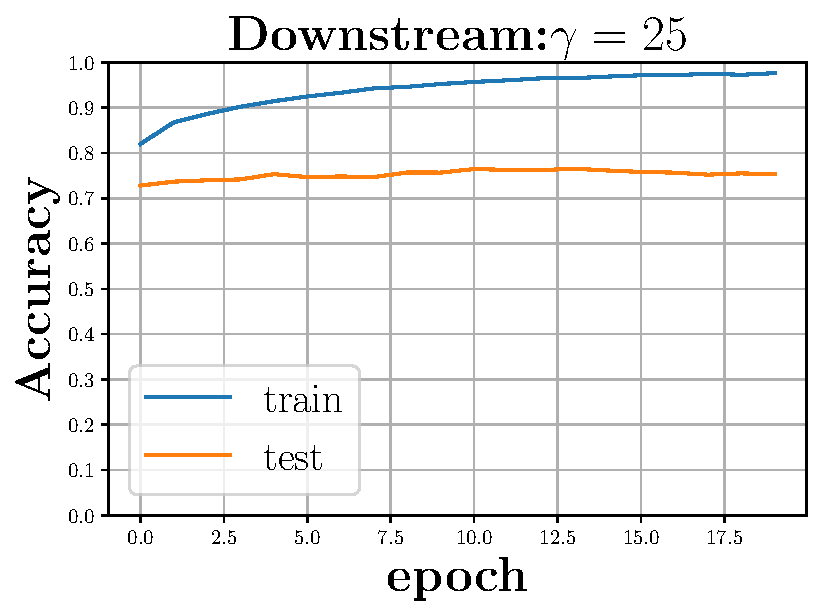
\includegraphics[scale=0.125]{figs/relu_25_good.pdf}&
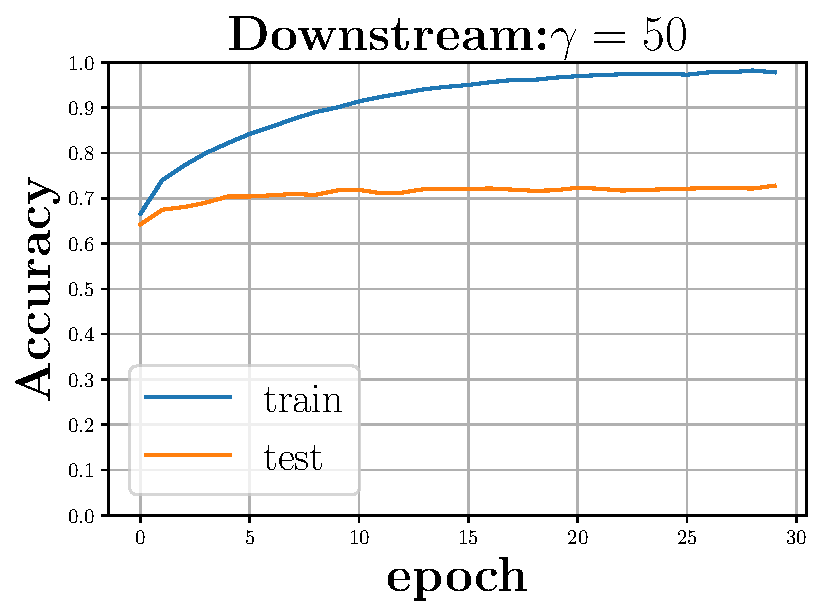
\includegraphics[scale=0.125]{figs/relu_50_good.pdf}&
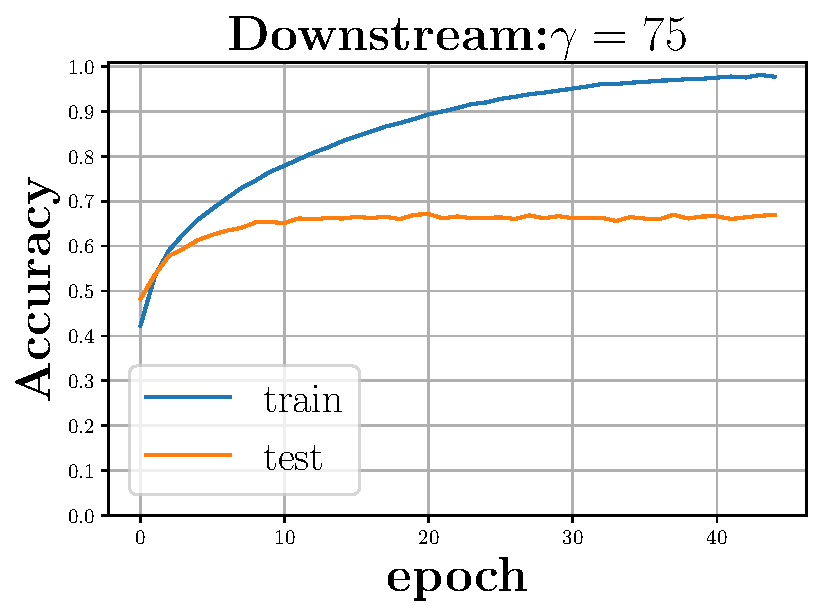
\includegraphics[scale=0.125]{figs/relu_75_good.pdf}\\
\end{tabular}
}
\end{minipage}
\caption{Shows the upstream training with random labels followed downstream training with true labels. The first epochs of bottom plots is same as the epoch follows the last epoch in the top plots.}
\label{fig:rand-label}

\end{figure}
\end{comment}

\begin{comment}
\begin{figure}[h]
%\begin{comment}
\begin{minipage}{0.4\columnwidth}
\resizebox{\columnwidth}{!}{
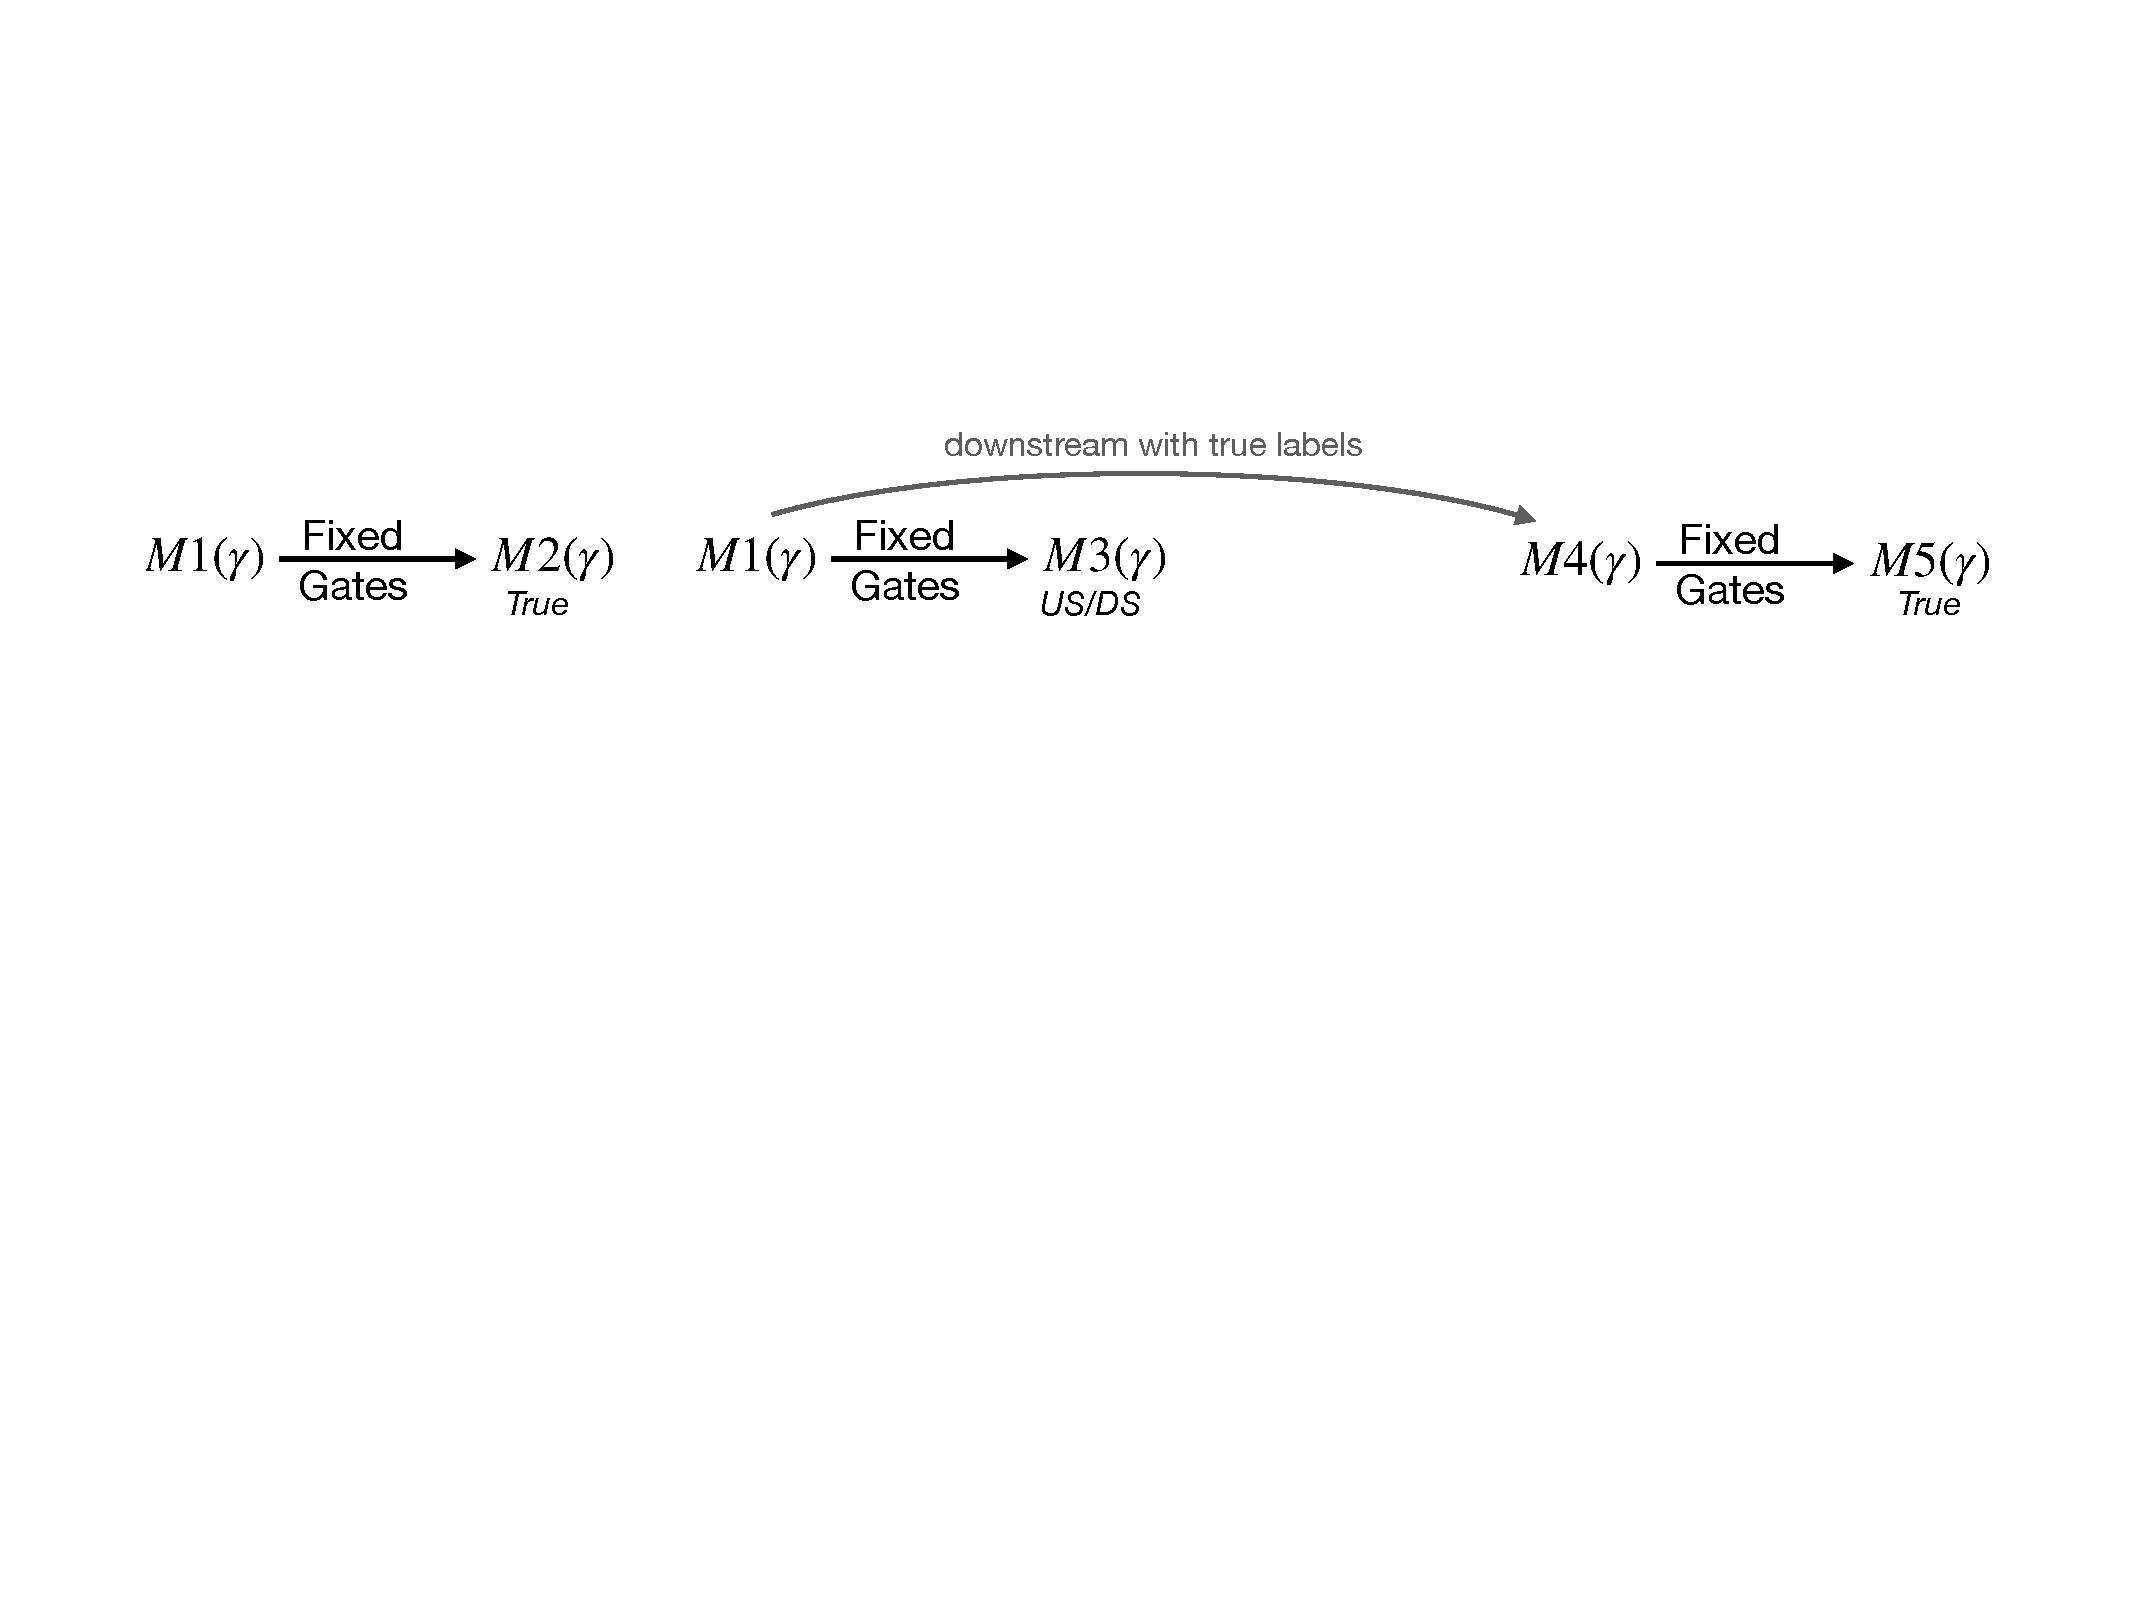
\includegraphics[scale=0.35]{figs/rand-label.pdf}
}
\end{minipage}
%\end{comment}
\begin{minipage}{0.99\columnwidth}
\resizebox{\columnwidth}{!}{
\begin{tabular}{cccccc}
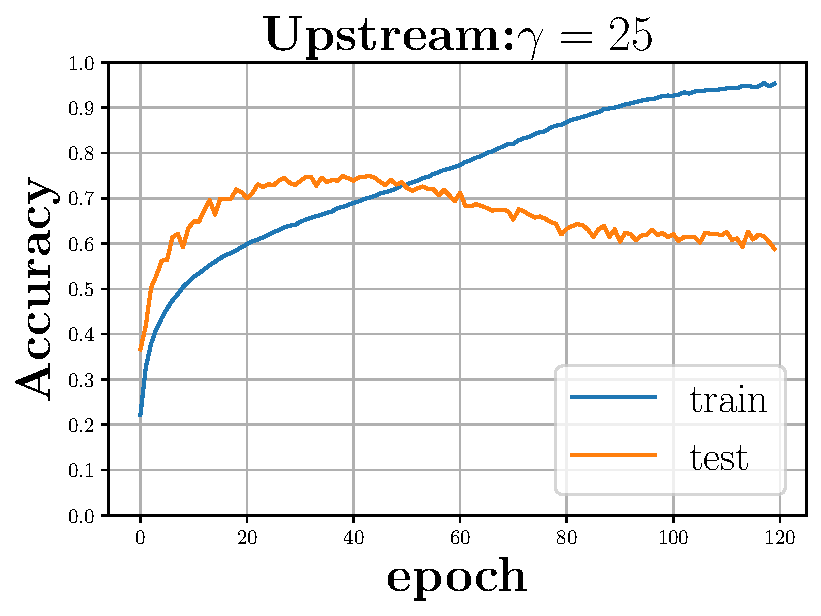
\includegraphics[scale=0.125]{figs/relu_25.pdf}&
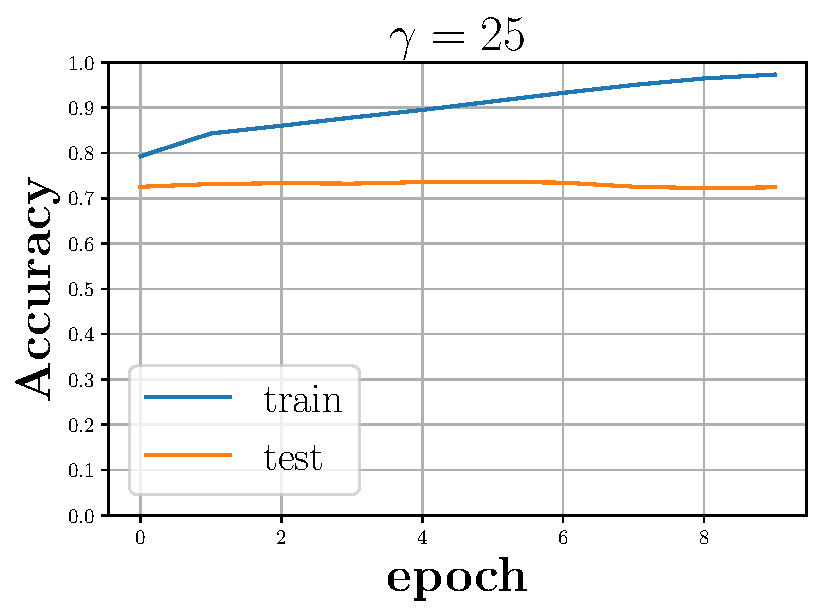
\includegraphics[scale=0.125]{figs/galu_25_good.pdf}&
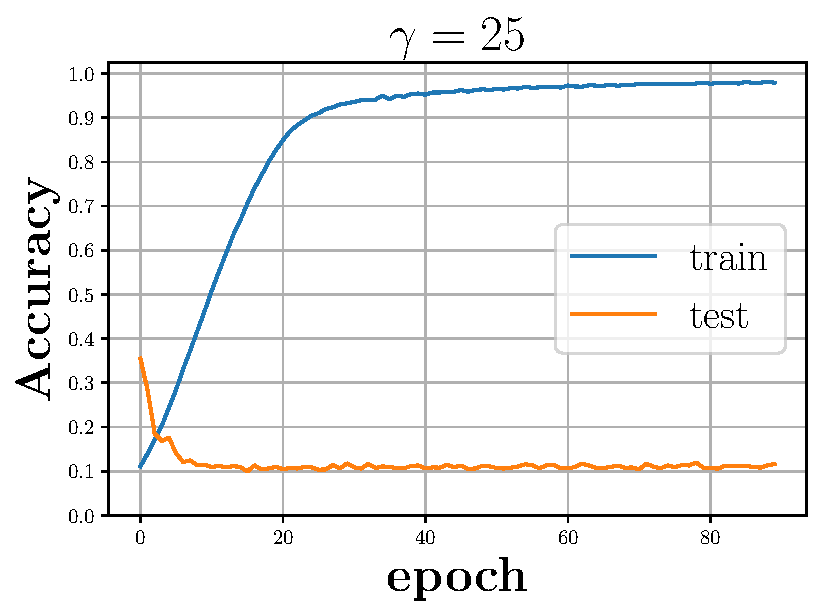
\includegraphics[scale=0.125]{figs/galu_25_bad.pdf}&
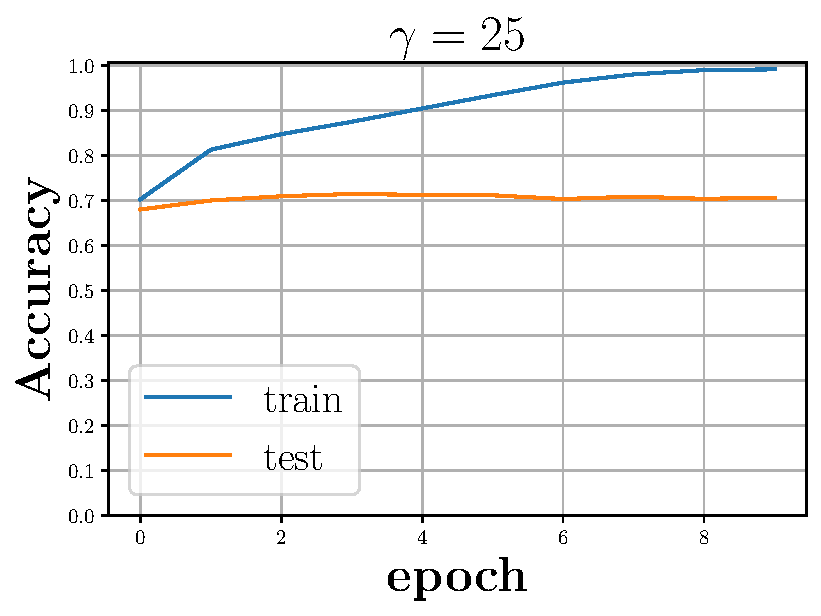
\includegraphics[scale=0.125]{figs/galu_25_bad_good.pdf}&
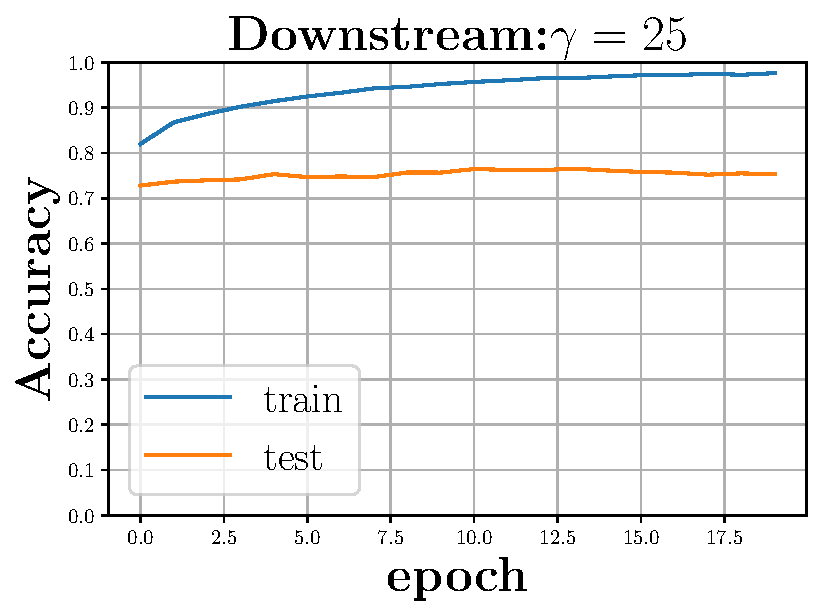
\includegraphics[scale=0.125]{figs/relu_25_good.pdf}&
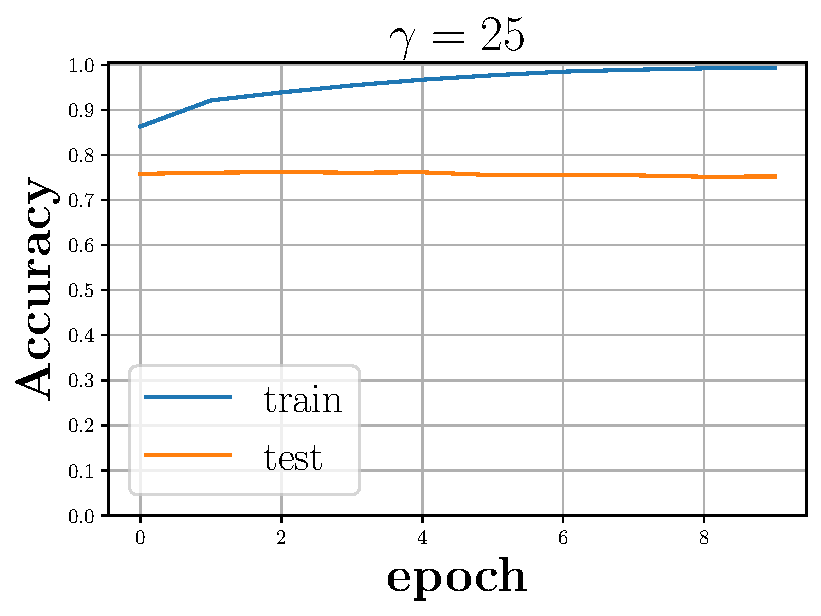
\includegraphics[scale=0.125]{figs/galu_25_recovered.pdf}
\\
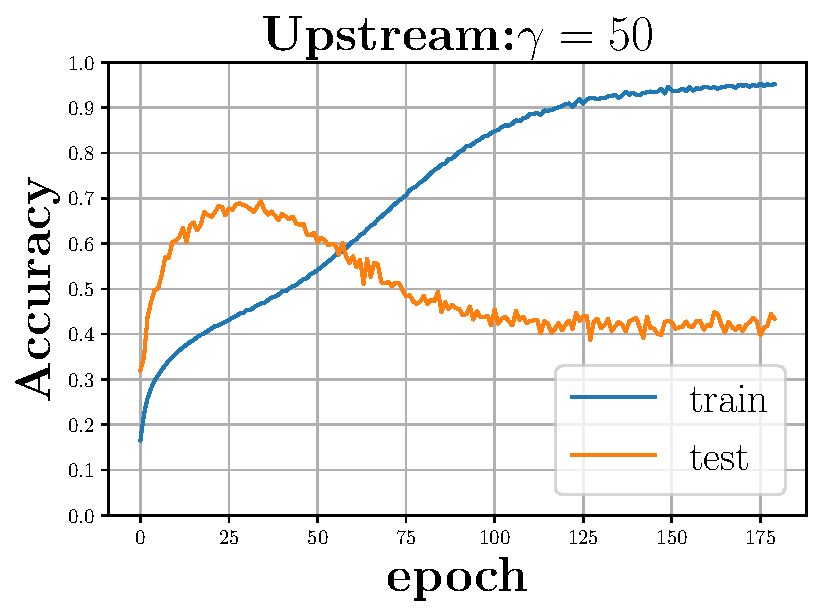
\includegraphics[scale=0.125]{figs/relu_50.pdf}&
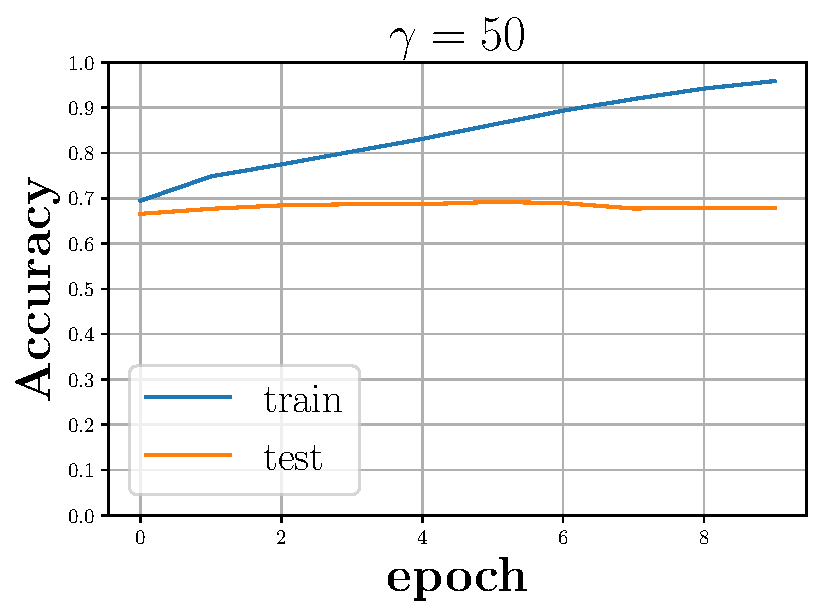
\includegraphics[scale=0.125]{figs/galu_50_good.pdf}&
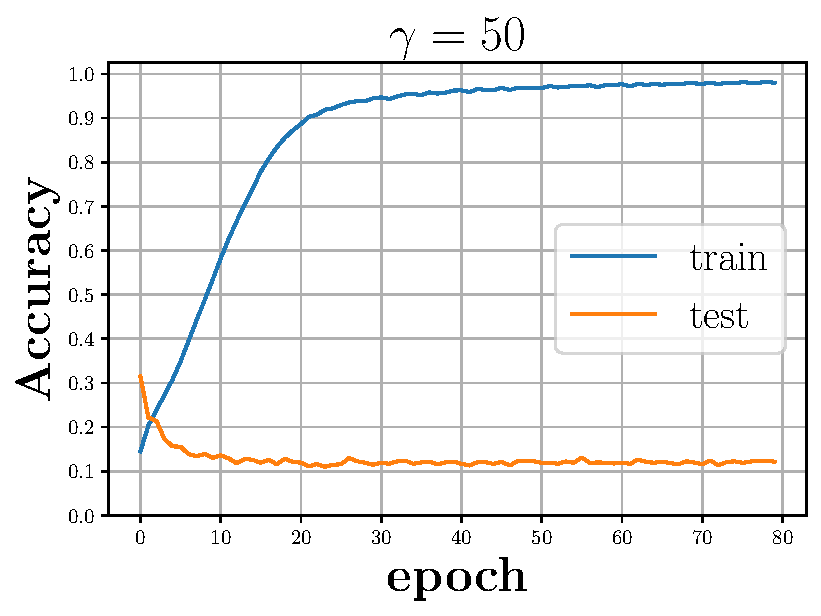
\includegraphics[scale=0.125]{figs/galu_50_bad.pdf}&
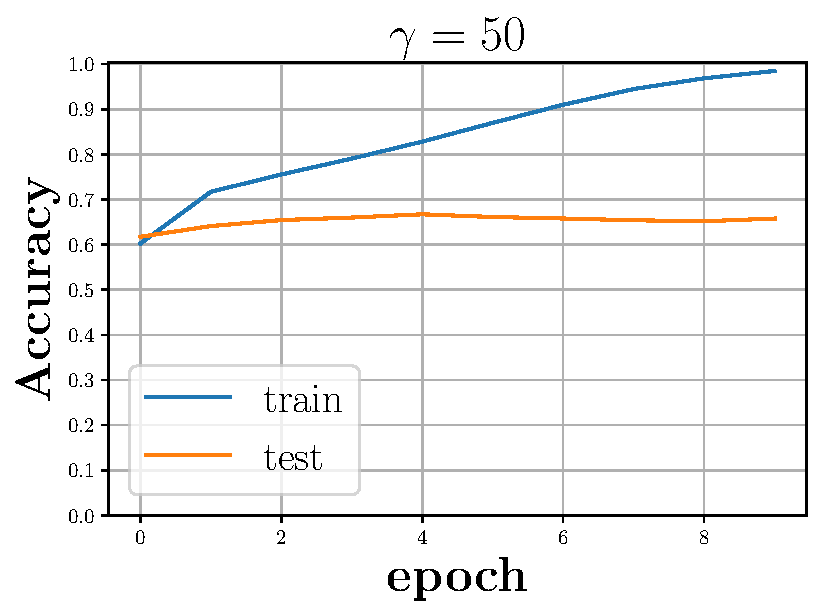
\includegraphics[scale=0.125]{figs/galu_50_bad_good.pdf}&
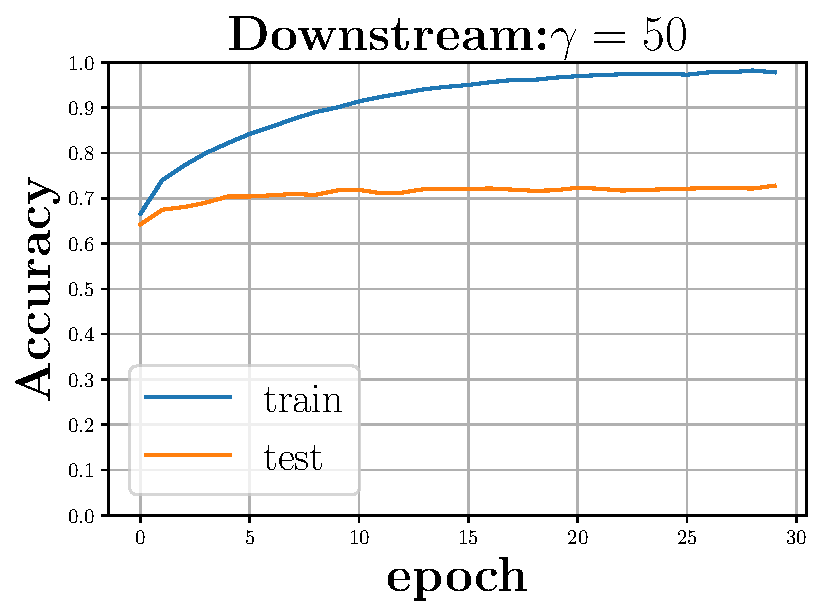
\includegraphics[scale=0.125]{figs/relu_50_good.pdf}&
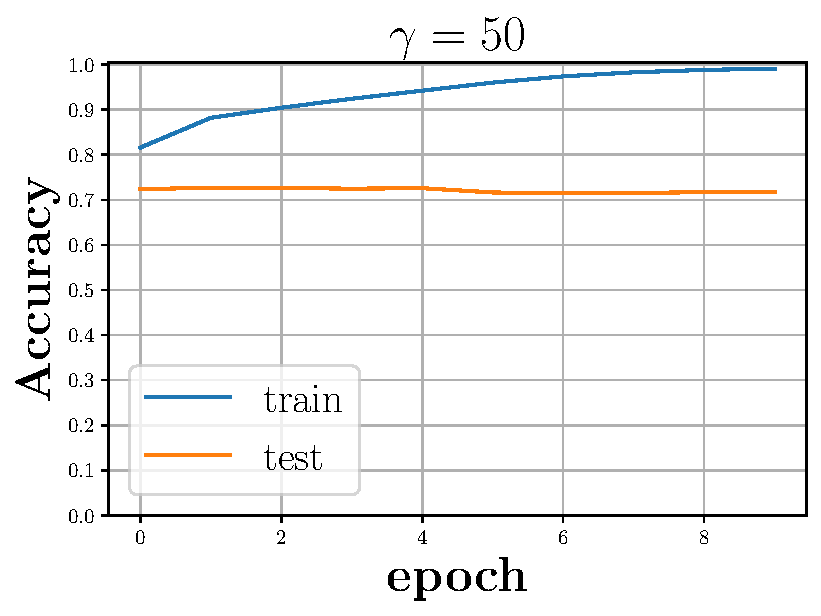
\includegraphics[scale=0.125]{figs/galu_50_recovered.pdf}
\\
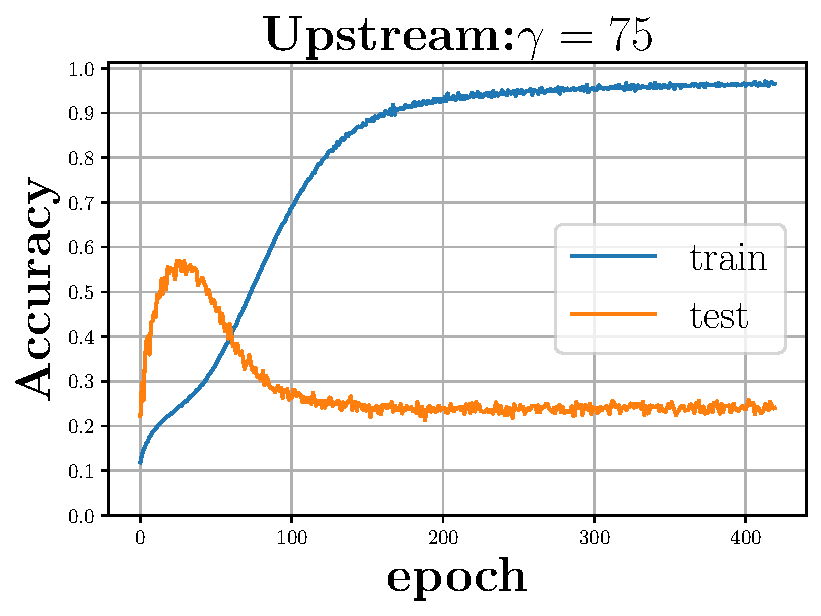
\includegraphics[scale=0.125]{figs/relu_75.pdf}&
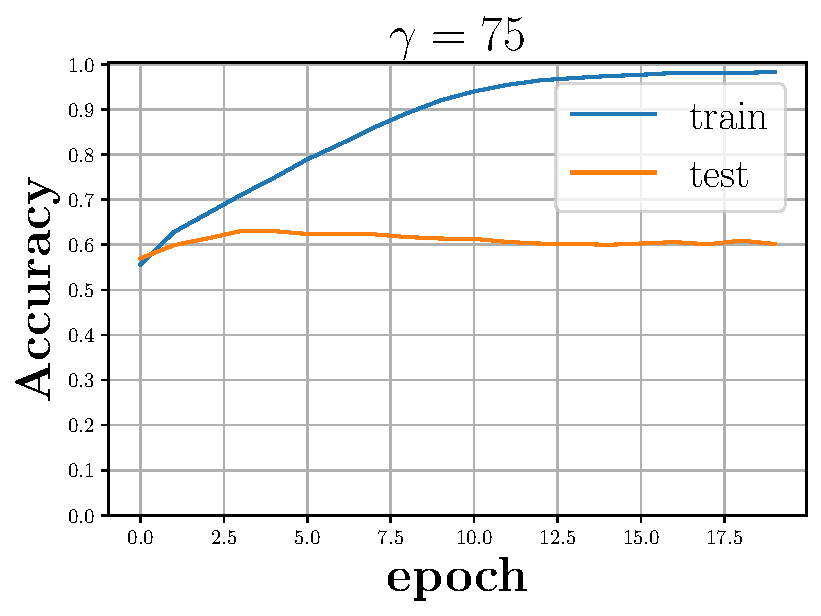
\includegraphics[scale=0.125]{figs/galu_75_good.pdf}&
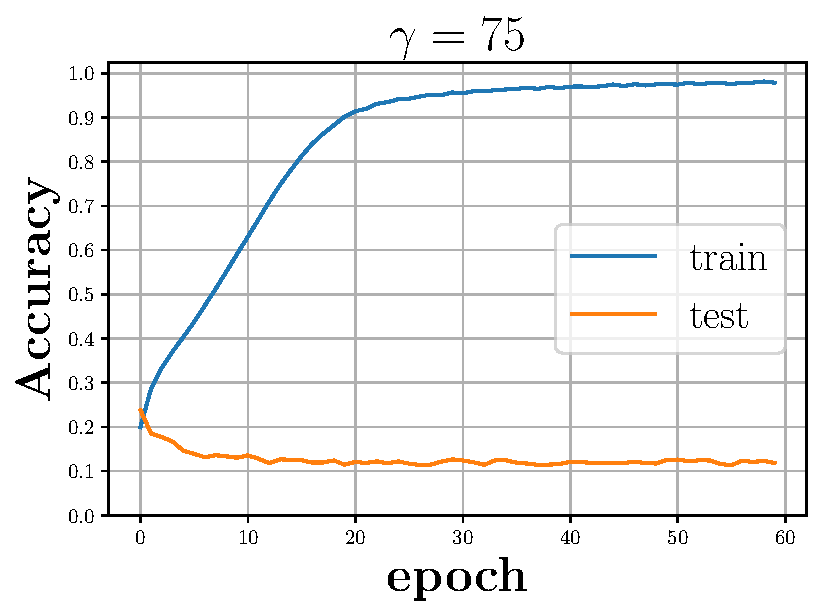
\includegraphics[scale=0.125]{figs/galu_75_bad.pdf}&
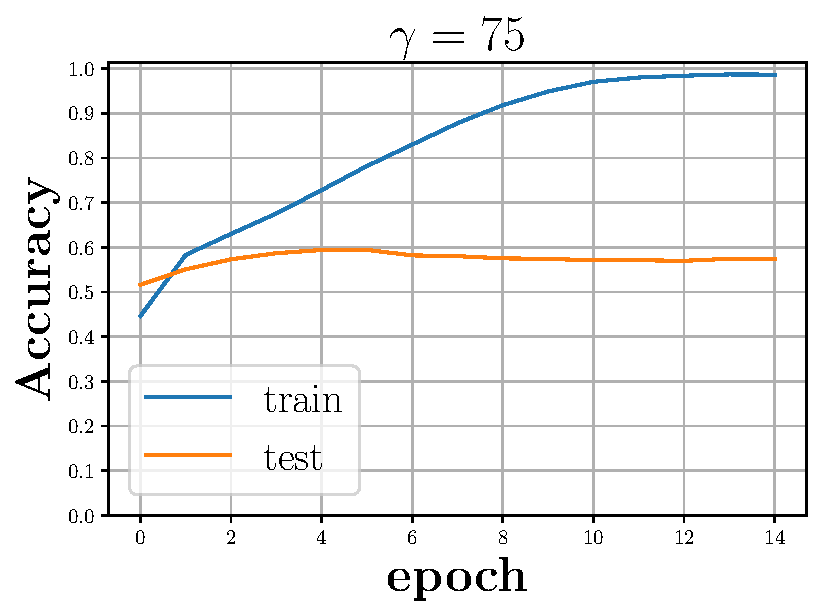
\includegraphics[scale=0.125]{figs/galu_75_bad_good.pdf}&
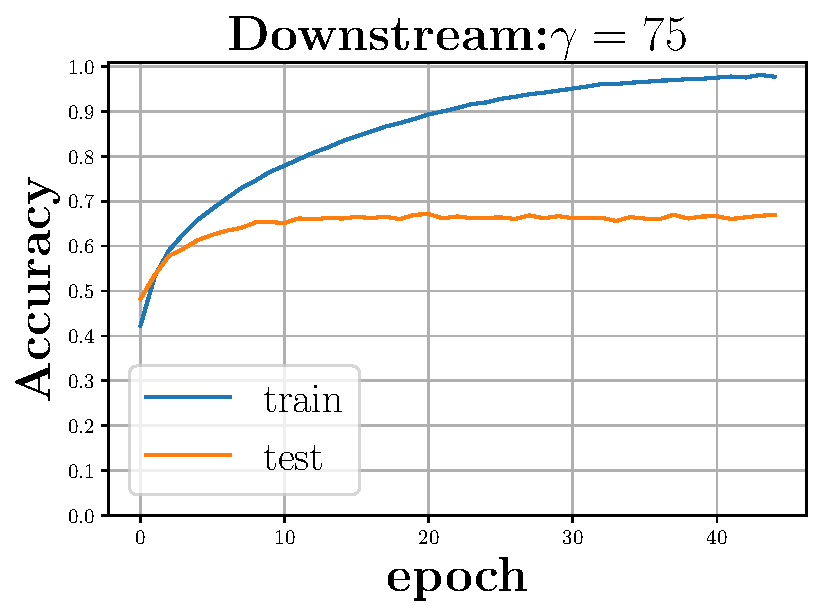
\includegraphics[scale=0.125]{figs/relu_75_good.pdf}&
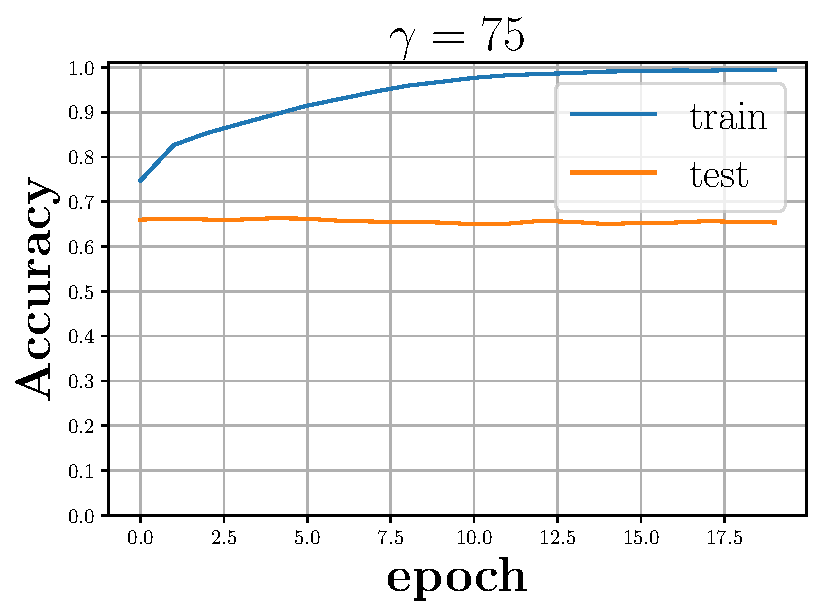
\includegraphics[scale=0.125]{figs/galu_75_recovered.pdf}\\
\tiny{M1}&\tiny{M2}&\tiny{M3:US}&\tiny{M3:DS}&\tiny{M4}&\tiny{M5}\\
\end{tabular}
}
\end{minipage}

\label{fig:rand-label}

\end{figure}

\end{comment}


\begin{comment}
\begin{figure}[h]
\begin{minipage}{0.40\columnwidth}
\begin{tabular}{|c|c|c|}\hline
ReLU& \multicolumn{2}{c|}{}\\
with   & \multicolumn{2}{c|}{Fixed Learnt Gates from }\\
 True &\multicolumn{2}{c|}{ReLU with True Labels}\\
Labels &  \multicolumn{2}{c|}{}\\\cline{2-3}
&True & {US/DS}\\\hline
 80.8& 80& 79\\\hline
 col-1 & col-2 & col-3\\\hline
\end{tabular}

\end{minipage}
\begin{minipage}{0.62\columnwidth}
\begin{tabular}{|c|c|c|c|c|c|c|c|}\hline
\%& \multicolumn{3}{c|}{\multirow{2}{*}{ReLU}} & \multicolumn{2}{c|}{FLG at End}&{FLG at End}\\
Label& \multicolumn{3}{c|}{{}} &\multicolumn{2}{c|}{of ReLU US}& of ReLU DS\\\cline{2-7}
Noise & \multicolumn{2}{c|}{Rand. US} & True & \multicolumn{1}{c|}{\multirow{2}{*}{True}} &{US/DS}& \multicolumn{1}{c|}{\multirow{2}{*}{True}} \\\cline{2-3}
{} & Best & End & DS &{} &  &\\\hline
25&75.3 & 63.1& 76.7&74.2 & 72.3& 76.5\\\hline
50& 69.8 &41.5&73.1&69.6 &67& 73.1\\\hline
 col-1 & col-2 & col-3&  col-4 & col-5 & col-6& col-7\\\hline
\end{tabular}
\end{minipage}
\end{figure}
\end{comment}

